\documentclass{beamer}[10]

\usepackage{graphicx}
\usepackage{xcolor}
\usepackage{tabto}
%\usepackage{beamerthemesplit}
\usepackage{tikz}
\usepackage{cancel}
\usepackage{verbatim}
\usepackage{fancybox}
\usepackage{enumerate}
\usepackage{amsmath,amssymb,amsthm,textcomp,mathtools}
\usepackage[super]{nth}
\usepackage[amssymb]{SIunits}
\usepackage{booktabs}
\usepackage{cancel}
\usepackage{bm}
\usepackage[utf8]{inputenc}
\usepackage{tabularx}
\usepackage{ragged2e}
\newcolumntype{Y}{ >{\RaggedRight\arraybackslash}X}
\usetikzlibrary{arrows,shapes}
\newcommand\T{\rule{0pt}{2.6ex}}
\newcommand\B{\rule[-1.2ex]{0pt}{0pt}}
\definecolor{UUcrimson}{RGB}{204,0,0}
\mode<presentation>
{ \usetheme{default}
  \usecolortheme[named=UUcrimson]{structure}
  \useinnertheme{circles}
  \setbeamercovered{transparent}
  \setbeamertemplate{blocks}[rounded]
  \usefonttheme[onlymath]{serif}
  \setbeamertemplate{navigation symbols}{}
  \setbeamertemplate{footline}[page number]
  \setbeamertemplate{navigation symbols}{}
  \setbeamercolor{section in toc}{fg=black,bg=white}
  \setbeamercolor{alerted text}{fg=UUcrimson!80!gray}
  \setbeamercolor*{palette primary}{fg=white,bg=UUcrimson}
  \setbeamercolor*{palette secondary}{fg=UUcrimson!70!black,bg=gray!15!white}
  \setbeamercolor*{palette tertiary}{bg=UUcrimson!80!black,fg=gray!10!white}
  \setbeamercolor*{palette quaternary}{fg=UUcrimson,bg=gray!5!white}
  \setbeamercolor*{palette sidebar primary}{fg=UUcrimson!10!black}
  \setbeamercolor*{palette sidebar secondary}{fg=white}
  \setbeamercolor*{palette sidebar tertiary}{fg=UUcrimson!50!black}
  \setbeamercolor*{palette sidebar quaternary}{fg=gray!10!white}
  \setbeamercolor{titlelike}{parent=palette primary,fg=white}
  \setbeamercolor{frametitle}{bg=UUcrimson}
  \setbeamercolor{frametitle right}{bg=UUcrimson}
  \setbeamercolor*{separation line}{}
  \setbeamercolor*{fine separation line}{}
}

\usetikzlibrary{backgrounds}
\makeatletter
\tikzstyle{every picture}+=[remember picture]
\tikzset{%
  fancy quotes/.style={
    text width=\fq@width pt,
    align=justify,
    inner sep=1em,
    anchor=north west,
    minimum width=\linewidth,
    font=\itshape
  },
  fancy quotes width/.initial={.8\linewidth},
  fancy quotes marks/.style={
    scale=8,
    text=white,
    inner sep=0pt,
  },
  fancy quotes opening/.style={
    fancy quotes marks,
  },
  fancy quotes closing/.style={
    fancy quotes marks,
  },
  fancy quotes background/.style={
    show background rectangle,
    inner frame xsep=0pt,
    background rectangle/.style={
      fill=gray!25,
      rounded corners,
    },
  }
}
\newenvironment{fancyquotes}[1][]{%
\noindent
\tikzpicture[fancy quotes background]
\node[fancy quotes opening,anchor=north west] (fq@ul) at (0,0) {``};
\tikz@scan@one@point\pgfutil@firstofone(fq@ul.east)
\pgfmathsetmacro{\fq@width}{\linewidth - 2*\pgf@x}
\node[fancy quotes,#1] (fq@txt) at (fq@ul.north west) \bgroup}
{\egroup;
\node[overlay,fancy quotes closing,anchor=east] at (fq@txt.south east) {''};
\endtikzpicture}
\makeatother


\usetikzlibrary{backgrounds}
\makeatletter
\tikzstyle{every picture}+=[remember picture]
\tikzset{%
  fancy defs/.style={
    text width=\fq@width pt,
    align=justify,
    inner sep=0.25em,
    anchor=north west,
    minimum width=\linewidth,
    font=\itshape
  },
  fancy defs width/.initial={.8\linewidth},
  fancy defs marks/.style={
    scale=8,
    text=white,
    inner sep=0pt,
  },
  fancy defs opening/.style={
    fancy defs marks,
  },
  fancy defs closing/.style={
    fancy defs marks,
  },
  fancy defs background/.style={
    show background rectangle,
    inner frame xsep=0pt,
    background rectangle/.style={
      fill=gray!25,
      rounded corners,
    },
  }
}
\newenvironment{fancydefs}[1][]{%
\noindent
\tikzpicture[fancy defs background]
\node[fancy defs opening,anchor=north west] (fq@ul) at (0,0) {};
\tikz@scan@one@point\pgfutil@firstofone(fq@ul.east)
\pgfmathsetmacro{\fq@width}{\linewidth - 2*\pgf@x}
\node[fancy defs,#1] (fq@txt) at (fq@ul.north west) \bgroup}
{\egroup;
\node[overlay,fancy defs closing,anchor=east] at (fq@txt.south east) {};
\endtikzpicture}
\makeatother
\usepackage{scalerel}[2014/03/10]
\usepackage{stackengine}
\usepackage{empheq}
\newcommand*\widefbox[1]{\fbox{\hspace{0.5em}#1\hspace{0.5em}}}

\newcommand\reallywidetilde[1]{\ThisStyle{%
  \setbox0=\hbox{$\SavedStyle#1$}%
  \stackengine{-.1\LMpt}{$\SavedStyle#1$}{%
    \stretchto{\scaleto{\SavedStyle\mkern.2mu\sim}{.5467\wd0}}{.4\ht0}%
%    .2mu is the kern imbalance when clipping white space
%    .5467++++ is \ht/[kerned \wd] aspect ratio for \sim glyph
  }{O}{c}{F}{T}{S}%
}}
\usepackage{media9}

\logo{
\includegraphics[width=0.75cm]{logo.jpg}}
\author[Gibbs]{Dr. Jeremy A. Gibbs}
\institute{Department of Mechanical Engineering\\University of Utah}
\date{Spring 2017}
\title{Environmental Fluid Dynamics: Lecture 5}
% colors
\definecolor{colororange}{HTML}{E65100} % orange
\definecolor{colordgray}{HTML}{795548} % dark gray for note
\definecolor{colorhgray}{HTML}{212121} % heavy dark gray for normal text
\definecolor{colorgreen}{HTML}{009688} % green
\definecolor{colorwhite}{HTML}{FFFFFF} % background white
\definecolor{colorlgray}{HTML}{F5F3EE} % background light gray
\definecolor{colorblue}{HTML}{0277BB} % blue
\definecolor{colorred}{HTML}{CC0000} % red
\newcommand{\fontsizeone}{1.9em}
\setbeamertemplate{caption}{\raggedright\insertcaption\par}
\newcommand{\framecard}[2][colorgreen]{
  {\setbeamercolor{background canvas}{bg=#1}
    \begin{frame}[plain]
    \vfill
    \begin{center}
     {#2}
    \end{center}
    \vfill
    \end{frame}
  }
}

\begin{document}

%----------------------------------------------------------------------------------------
%	TITLE & TOC SLIDES
%----------------------------------------------------------------------------------------

\begin{frame} 
  \titlepage
\end{frame}

%------------------------------------------------

\begin{frame}
\frametitle{Overview}
\tableofcontents
\end{frame}

%------------------------------------------------
\section{Atmospheric Thermodynamics} %
%------------------------------------------------
\framecard[colorred]{{\color{white}\Huge Atmospheric Thermodynamics}}
%------------------------------------------------
\subsection{Hypsometric Equation}
%------------------------------------------------

\begin{frame}{Atmospheric Thermodynamics: Hypsometric Equation}
\begin{itemize}
	\item Recall from last class that the geopotential thickness between two pressure levels is
	$$Z_2 - Z_1 = \frac{R_d}{g_0} \int^{p_1}_{p_2} T_v \frac{dp}{p}$$
	\item If we assume the atmosphere is \textbf{isothermal} and neglect the virtual temperature correction
	$$Z_2 - Z_1 = H\ln\left(\frac{p_1}{p_2}\right)$$
	where
	$$H\equiv\frac{RT}{g_0} = 29.3T$$
	is the \textbf{scale height}
\end{itemize}
\end{frame}
%------------------------------------------------

\begin{frame}{Atmospheric Thermodynamics: Hypsometric Equation}
\begin{itemize}
	\item Scale height
	\begin{fancydefs}
		The height within which some parameter, such as pressure or density, decreases by a factor 1/$e$ in an isothermal atmosphere
	\end{fancydefs}
	\item We can see this by rearranging the thickness equation
	$$Z_2 - Z_1 = H\ln\left(\frac{p_1}{p_2}\right) \Rightarrow p_2 = p_1\exp\left[-\frac{(Z_2-Z_1)}{H}\right]$$
	\item So, $H$ may be thought of as a measure of the effective ``thickness'' of an atmospheric layer
\end{itemize}
\end{frame}

%------------------------------------------------

\begin{frame}{Atmospheric Thermodynamics: Hypsometric Equation}
\begin{figure}
	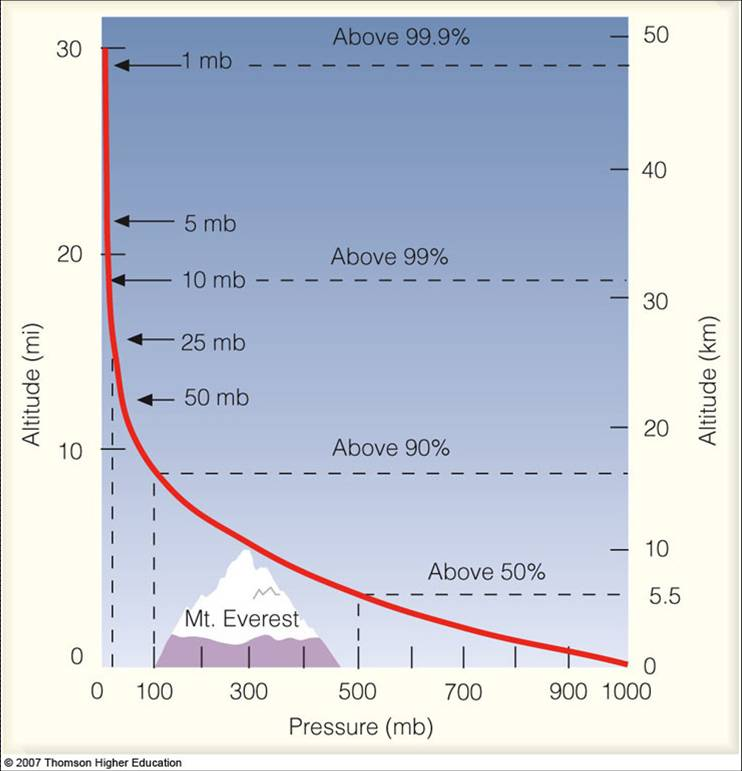
\includegraphics[height=0.88\textheight]{fig1}
\end{figure}
\end{frame}

%------------------------------------------------

\begin{frame}{Atmospheric Thermodynamics: Hypsometric Equation}
\begin{itemize}
	\item As we discussed earlier, temperature usually will vary with height
	\item It is not always appropriate to neglect the virtual temperature correction
	\item A more general approach is to integrate $T_v$ w.r.t. presure as 
	$$\bar T_v \equiv \cfrac{\int^{p_1}_{p2} T_v d(\ln{p})}{\int^{p_1}_{p2} d(\ln{p})} = \cfrac{\int^{p_1}_{p2} T_v \cfrac{dp}{p}}{\ln{\left(\cfrac{p_1}{p_2}\right)}}$$
	\item Which leads to the \textbf{hypsometric equation}
	$$Z_2 - Z_1 = \bar H\ln\left(\frac{p_1}{p_2}\right) = \frac{R_d\bar T_v}{g_0}\ln\left(\frac{p_1}{p_2}\right)$$
\end{itemize}
\end{frame}

%------------------------------------------------
\subsection{Reducing Pressure to Seal Level}
%------------------------------------------------

\begin{frame}{Atmospheric Thermodynamics: Reducing P to SLP}
\begin{itemize}
	\item In areas with mountainous terrain, changes in surface pressure between one site and another are largely caused by differences in elevation
	\item We reduce surface pressure to a common level in order to separate the portion of the pressure field caused by weather
	\item  For a layer between the Earth's surface and sea level:
	$$Z_g = \overline{H}\ln{\left(\frac{p_0}{p_g}\right)}$$
	\item We can use this to solve for sea-level pressure (SLP)
	$$p_0 = p_g\exp{\left(\frac{Z_g}{\overline{H}}\right)} = p_g \exp{\left(\frac{g_0Z_g}{R_d\overline{T}_v}\right)}$$
\end{itemize}
\end{frame}
%------------------------------------------------

\begin{frame}{Atmospheric Thermodynamics: Reducing P to SLP}
$$p_g \exp{\left(\frac{g_0Z_g}{R_d\overline{T}_v}\right)}$$
\begin{itemize}
	\item if $Z_g/\overline{H} \ll 1$, then $\exp{\left(Z_g/\overline{H}\right)}\sim 1+Z_g/\overline{H}$ and we can rewrite as
	$$p_0 - p_g \simeq p_g\frac{Z_g}{\overline{H}} = p_g\left(\frac{g_0 Z_g}{R_d \overline{T}_v}\right)$$
	\item If we use representative values of $p_g\simeq1000\ \hecto\pascal$ and $\overline{H} \simeq 8000\ \metre$, then the pressure correction is
	$$p_0 - p_g \sim \frac{Z_g}{8}$$
	This means that pressure decreases by $1\ \hecto\pascal$ every $8\ \metre$ of ascent (within first couple hundred meters above/below SLP)
\end{itemize}
\end{frame}
%------------------------------------------------
\subsection{\nth{1} Law of Thermodynamics}
%------------------------------------------------
\begin{frame}{Atmospheric Thermodynamics: \nth{1} Law of Thermo}
\begin{itemize}
	\item Imagine a closed system of unit mass
	\item Thermal energy $Q$ ($\joule$) is added to the system via conduction and/or radiation
	\item In response, the system may do some amount of external work $W$
	\item The excess energy given to body over the external work done by the body is given by $Q-W$
\end{itemize}
\end{frame}
%------------------------------------------------
\begin{frame}{Atmospheric Thermodynamics: \nth{1} Law of Thermo}
\begin{itemize}
	\item It follows from conservation of energy that the internal energy of the system must increase by $Q-W$, or
	$$dQ - dW = dU$$
	where
	\begin{itemize}
		\item $dQ \rightarrow$ differential heat added to system
		\item $dW \rightarrow$ differential work done by system
		\item $dU \rightarrow$ differential increase in internal energy
	\end{itemize}
	\item This describes4 the \textbf{First Law of Thermodynamics}
	\item The change in internal energy only depends on the initial and final states of the system - and not the transfer mechanism
\end{itemize}
\end{frame}

%------------------------------------------------
\begin{frame}{Atmospheric Thermodynamics: \nth{1} Law of Thermo}
\textbf{Joule's Law}
\begin{fancydefs}
	The internal energy of a fixed mass of an ideal gas depends only on its temperature (not pressure or volume)
\end{fancydefs}
\begin{itemize}
	\item Found that if a gas expands without doing external work and without taking/giving heat, then the temperature does not change
	\item This is only possible if molecules of an ideal gas do not exert forces on each other
\end{itemize}
\end{frame}
%------------------------------------------------
\begin{frame}{Atmospheric Thermodynamics: \nth{1} Law of Thermo}
\begin{itemize}
	\item Imagine heat $dQ$ is given to a unit mass, which causes the temperature to increase from $T$ to $T+dT$
	\item $dQ/dT \rightarrow$ \textbf{specific heat}
	\item If volume is held constant, then
	$$c_v = \left(\frac{dQ}{dT}\right)_{\text{v const}}$$
	\item Also if volume is constant, $dW=0$, which means $dQ=dU$:
	$$c_v = \left(\frac{dU}{dT}\right)_{\text{v const}}$$
	\item Invoking Joule's Law means $U$ only depends on $T$, so
	$$c_v = \left(\frac{dU}{dT}\right)$$
\end{itemize}
\end{frame}
%------------------------------------------------
\begin{frame}{Atmospheric Thermodynamics: \nth{1} Law of Thermo}
\begin{itemize}
	\item The First Law of Thermodynamics for an ideal gas
	$$dQ = c_vdT + pd\alpha$$
	where $\alpha = 1/\rho$ is specific volume
	\item Adding heat will either change $T$ or $\alpha$
	\item The change in $U$ is given by
	$$dU = \int^{T_2}_{T_1} c_v dT$$
\end{itemize}
\end{frame}
%------------------------------------------------
\begin{frame}{Atmospheric Thermodynamics: \nth{1} Law of Thermo}
\begin{itemize}
	\item We can also define a specific heat at \textit{constant pressure}
	$$c_p = \left(\frac{dQ}{dT}\right)_{\text{p const}}$$
	\item Here, heat is added, temperature rises, and the system expands - but the pressure remains constant
	\item Some amount of the heat added to the system is expended to expand against constant pressure of environment
	\item Thus, more heat must be added to raise a material's temperature by a given amount than if volume had been kept constant
\end{itemize}
\end{frame}
%------------------------------------------------
\begin{frame}{Atmospheric Thermodynamics: \nth{1} Law of Thermo}
$$dQ = c_vdT + pd\alpha$$
\begin{itemize}
	\item Using product rule, $d(p\alpha) = pd\alpha + \alpha dp$, so
	$$dQ = c_vdT + d(p\alpha) - \alpha dp$$
	\item Recall ideal gas law
	$$p\alpha = RT$$
	so
	$$d(p\alpha) = d(RT) = RdT + \cancelto{0}{TdR} = RdT$$
	\item We can rewrite as
	$$dQ = c_vdT + RdT - \alpha dp = (c_v + R)dT - \alpha dp$$ 
\end{itemize}
\end{frame}
%------------------------------------------------
\begin{frame}{Atmospheric Thermodynamics: \nth{1} Law of Thermo}
$$dQ = (c_v + R)dT - \alpha dp$$ 
\begin{itemize}
	\item At constant pressure, $\alpha dp = 0$, so
	\begin{align*}
	dQ &= (c_v + R)dT\\
	\left(\frac{dQ}{dT}\right)_{\text{p const}} &= c_v + R\\
	\Aboxed{c_p &= c_v + R}
	\end{align*}
\end{itemize}
\end{frame}
%------------------------------------------------
\begin{frame}{Atmospheric Thermodynamics: \nth{1} Law of Thermo}
\begin{itemize}
	\item For dry air, $c_v=717\ \joule\ \reciprocal\kelvin\ \kilo\reciprocal\gram$ and $c_p=1004\ \joule\ \reciprocal\kelvin\ \kilo\reciprocal\gram$
	\item Note that $1004\ \joule\ \reciprocal\kelvin\ \kilo\reciprocal\gram-717\ \joule\ \reciprocal\kelvin\ \kilo\reciprocal\gram = 287\ \joule\ \reciprocal\kelvin\ \kilo\reciprocal\gram$, which is the gas constant for dry air $R_d$
	\item Using $c_p = c_v + R$ and $dQ = (c_v + R)dT$, we can rewrite the First Law of Thermodynamics as
	$$dQ = c_pdT - \alpha dp$$
	\item So, in terms of specific heat, we have
	\begin{align*}
		dQ &= c_vdT + pd\alpha\\
		dQ &= c_pdT - \alpha dp
	\end{align*}
\end{itemize}
\end{frame}
%------------------------------------------------
\begin{frame}{Atmospheric Thermodynamics: \nth{1} Law of Thermo}
\begin{itemize}
	\item Imagine heat is added to a material at constant $p$ such that $\alpha$ increases
	\item The work done my a unit mass of the material is $p(\alpha_2 -\alpha_1)$
	\item Thus, the finite heat added to a unit mass at constant pressure is
	$$\Delta Q = (U_2-U_1) + p(\alpha_2 -\alpha_1) = (u_2+p\alpha_2) -(u_1+p\alpha_1)$$
	\item We can rewrite this as
	$$\Delta Q = H_2 - H_1$$
	where $H \equiv U+p\alpha$ is the \textbf{enthalpy}
\end{itemize}
\end{frame}
%------------------------------------------------
\begin{frame}{Atmospheric Thermodynamics: \nth{1} Law of Thermo}
$$H \equiv U+p\alpha$$
\begin{itemize}
	\item Integrating our expression for enthalpy gives
	$$dH=dU + d(p\alpha)$$
	\item Recall that $c_v = (dU/dT)$ and $dQ = c_vdT + d(p\alpha) - \alpha dp$, so $dU=c_vdT=dQ-d(p\alpha)+\alpha dp$
	\item We can combine
	\begin{align*}
		dH &= dU + d(p\alpha)\\
		&= dQ-d(p\alpha)+\alpha dp +d(p\alpha)\\
		&= dQ+\alpha dp
	\end{align*}
	which gives another form of the First Law of Thermodynamics
	$$dQ = dH - \alpha dp$$
\end{itemize}
\end{frame}
%------------------------------------------------
\begin{frame}{Atmospheric Thermodynamics: \nth{1} Law of Thermo}
$$dQ = dH - \alpha dp$$
\begin{itemize}
	\item Recall, $dQ = c_pdT - \alpha dp$
	\item Comparing with the enthalpy version above, we see that
	$$dH = c_pdT$$
	or if integrated
	$$H=c_pT$$
	where $h=0$ when $T=0$
	\item Thus, $H$ is the heat required to raise the temperature of a material from $0\ \kelvin$ to $T\ \kelvin$ at constant pressure
\end{itemize}
\end{frame}
%------------------------------------------------
\begin{frame}{Atmospheric Thermodynamics: \nth{1} Law of Thermo}
\begin{itemize}
	\item Imagine some slice of air is at rest and in hydrostatic balance
	\item If that slice is heated (radiative transfer), then the weight of the overlying air remains constant
	\item \textit{i.e.}, the heating is at constant pressure
	\item The increased energy added to the air appears in the form of an increase in enthalpy
	\item In atmospheric science, enthalpy is referred to as \textit{sensible heat}
\end{itemize}
\end{frame}
%------------------------------------------------
\begin{frame}{Atmospheric Thermodynamics: \nth{1} Law of Thermo}
\begin{itemize}
	\item In the case of heating at constant pressure ($\alpha dp=0$), we have
	$$dQ = dH = c_pdT$$
	\item This slice of air expands as it is heated, which results in work by pushing up the overlying air against gravity
	\item Recall $dQ = c_vdT + pd\alpha$, so for the energy given to the air, $c_vdT$ is the increase in internal energy and $pd\alpha=RdT$ is the work done on the overlying air
\end{itemize}
\end{frame}
%------------------------------------------------
\subsection{Adiabatic Processes}
%------------------------------------------------
\begin{frame}{Atmospheric Thermodynamics: Adiabatic Processes}
\textbf{Adiabatic Process}
\begin{fancydefs}
	When a material undergoes a physical state change (pressure, volume, temperature) without any heat exchange
\end{fancydefs}
\begin{itemize}
	\item So, $dQ=0$ for an adiabatic process
	\item Thus, for $dQ = c_vdT + pd\alpha$, we have
	$$-c_vdT = pd\alpha$$
	\item This means that expansion (compression) requires $dT<0$ ($dT>0$) or reduction (increase) in internal energy
\end{itemize}
\end{frame}
%------------------------------------------------
\begin{frame}{Atmospheric Thermodynamics: Adiabatic Processes}
\begin{columns}[T]
    \begin{column}{.4\textwidth}
    \begin{minipage}[c][0.8\textheight][c]{\linewidth}
    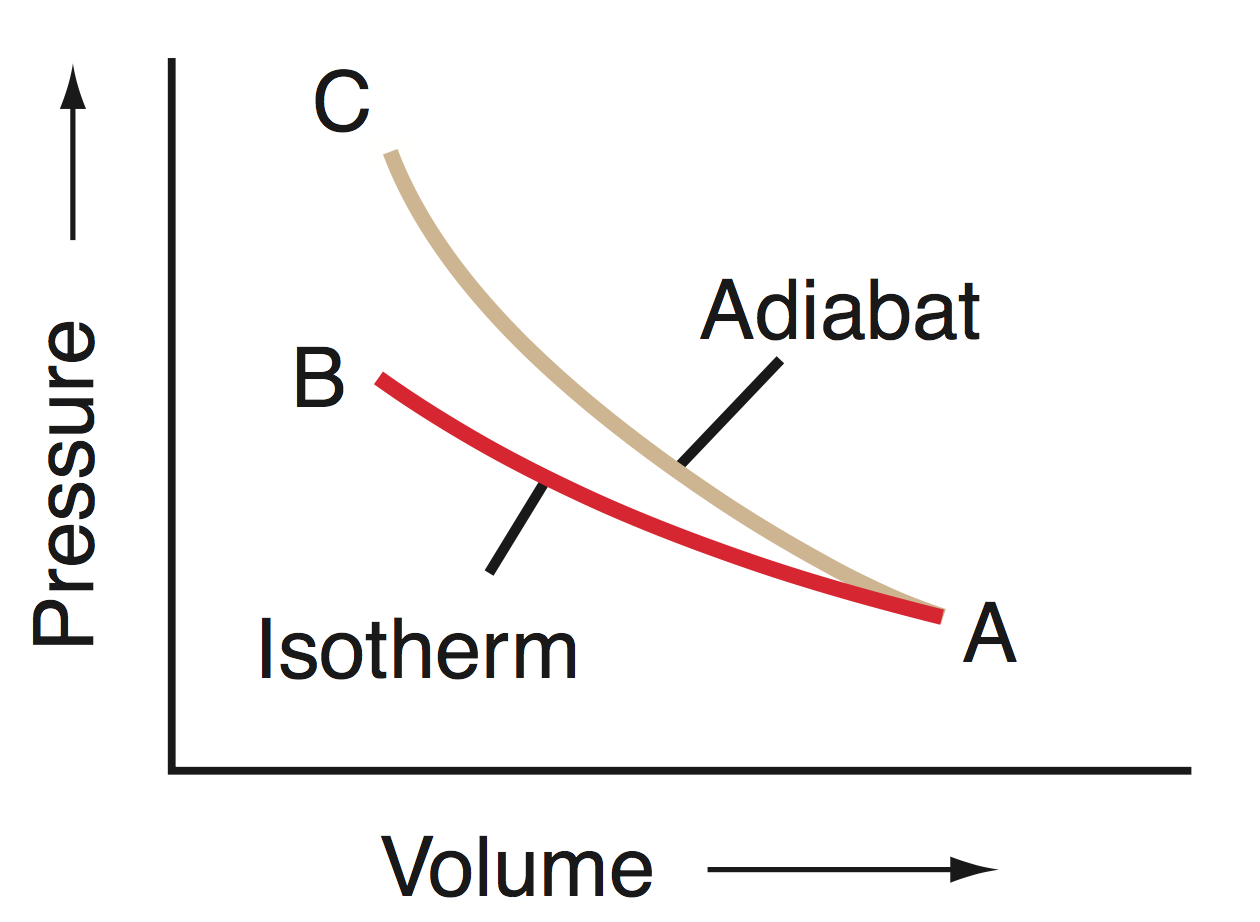
\includegraphics[width=1\textwidth]{fig2}\\
    \centering \small From Wallace and Hobbs (2006)
    \end{minipage}
    \end{column}
    \begin{column}{.6\textwidth}
    \begin{minipage}[c][0.8\textheight][c]{\linewidth}
   \begin{itemize}
   	\item Consider initial state at point A
   	\item An isothermal change is AB
   	\item A similar change in volume under adiabatic conditions is AC (called an adiabat)
   \end{itemize}
      \end{minipage}
    \end{column}
  \end{columns} 
\end{frame}
%------------------------------------------------
\begin{frame}{Atmospheric Thermodynamics: Adiabatic Processes}
\begin{columns}[T]
    \begin{column}{.4\textwidth}
    \begin{minipage}[c][0.8\textheight][c]{\linewidth}
    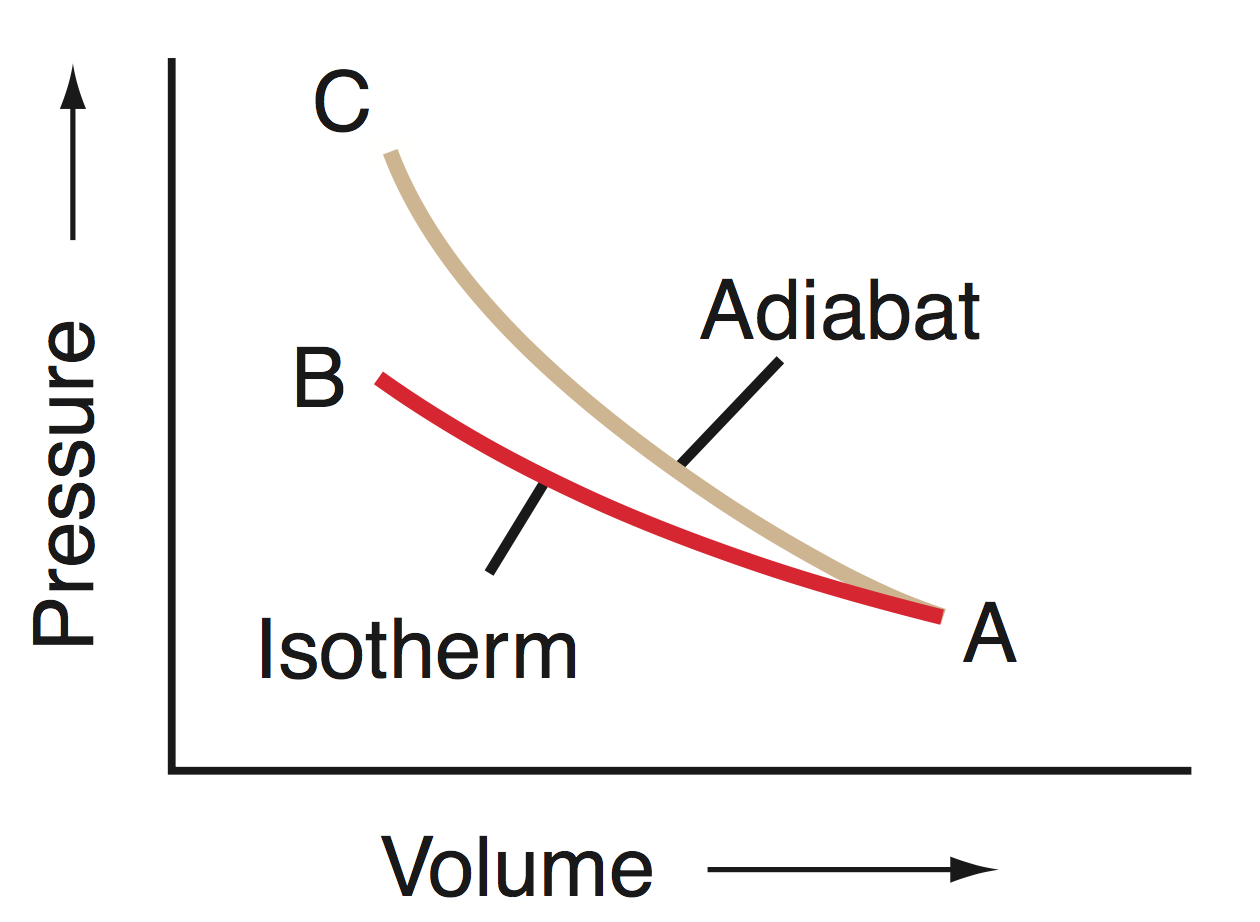
\includegraphics[width=1\textwidth]{fig2}\\
    \centering \small From Wallace and Hobbs (2006)
    \end{minipage}
    \end{column}
    \begin{column}{.6\textwidth}
    \begin{minipage}[c][0.8\textheight][c]{\linewidth}
   \begin{itemize}
   	\item Why is AC steeper?
   	\item Recall $dQ=0$, and we have $c_vdT = -pd\alpha$
   	\item For compression, $pd\alpha<0$, so $dT>0$
   	\item Conversely, for AB the temperature remains constant
   	\item Thus, $T_C>T_B$ and $p_C>p_B$
   \end{itemize}
      \end{minipage}
    \end{column}
  \end{columns} 
\end{frame}
%------------------------------------------------
\begin{frame}{Atmospheric Thermodynamics: Adiabatic Processes}
\begin{itemize}
	\item Mixing is often viewed as a result the random motions of individual molecules for many fluid dynamics applications
	\item However, molecular mixing in the atmosphere is only relevant in the lowest $\centi\metre$ or at $>105\ \kilo\metre$
	\item In between, vertical mixing is generally is accomplished by larger scale ``air parcels''
	\item We will use \textit{parcel theory} to try and better understand vertical mixing in the atmosphere
\end{itemize}
\end{frame}
%------------------------------------------------
\begin{frame}{Atmospheric Thermodynamics: Adiabatic Processes}
Assumptions for an air parcel of infinitesimal dimension
\begin{itemize}
	\item Thermally insulated - temperature changes adiabatically as it moves vertically
	\item Thus, the parcel pressure remains equal to the environmental pressure - which is assumed to be in hydrostatic balance
	\item Moves slowly enough such that macroscopic kinetic energy is a negligible fraction of its total energy
\end{itemize}
~\\~\\
So, if we lift an air parcel adiabatically (no transfer of energy across its surface) and bring it back to its original location then the pressure of the parcel will be the same - a \textbf{reversible process}
~\\~\\
In the real world these conditions are likely violated due to radiation and condensation
\end{frame}
%------------------------------------------------
\begin{frame}{Atmospheric Thermodynamics: Adiabatic Processes}
\textbf{Dry Adiabatic Lapse Rate}
\begin{fancydefs}
	The rate of change of temperature with height of a parcel of dry air that satisfies the assumptions of adiabatic mixing
\end{fancydefs}
\begin{itemize}
	\item Recall $dQ = c_pdT - \alpha dp$
	\item Since $dQ=0$, we get $c_pdT = \alpha dp$
	\item This leads to $dT/dp = \alpha/c_p = 1/(\rho c_p)$
	\item Making use of the hydrostatic equation $dp=-\rho g dz$
	$$-\frac{dT}{\rho g dz} = \frac{1}{\rho c_p}$$
	\item Rearranging yields
	$$\frac{dT}{dz} = -\frac{g}{c_p}$$
\end{itemize}
\end{frame}
%------------------------------------------------
\begin{frame}{Atmospheric Thermodynamics: Adiabatic Processes}
$$\frac{dT}{dz} = -\boxed{\frac{g}{c_p}}$$
\begin{itemize}
	\item Let's look at units of $g/c_p$
	$$\frac{[\metre\ \second\rpsquared]}{[\joule\ \reciprocal\kelvin\ \kilo\reciprocal\gram]} = \frac{[\metre\ \second\rpsquared]}{[\kilo\gram\ \metre\squared\ \second\rpsquared\ \reciprocal\kelvin\ \kilo\reciprocal\gram]} = \frac{[\kelvin]}{[\metre]}$$
	\item It is the \textbf{dry adiabatic lapse rate} $\Gamma_d$
	$$ \frac{dT}{dz} = -\Gamma_d$$
\end{itemize}
\end{frame}
%------------------------------------------------
\begin{frame}{Atmospheric Thermodynamics: Adiabatic Processes}
$$ \frac{dT}{dz} = -\Gamma_d$$
\begin{itemize}
	\item In the lowest $10\ \kilo\metre$, $g$ does not change much (see last lecture) and so $\Gamma_d$ is approximately constant 
	\item At sea level
	$$\Gamma_d = \frac{9.81\ \metre\ \second\rpsquared}{1004\ \joule\ \reciprocal\kelvin\ \kilo\reciprocal\gram} = 0.0098\ \kelvin\ \reciprocal\metre = 9.8\ \kelvin\ \kilo\reciprocal\metre$$
	\item Again, this is based on assuming adiabatic lifting/lowering - not something that really happens the atmosphere exactly
	\item Measurements indicate true lapse rate in the troposphere as
	$$\Gamma = \frac{\partial T}{\partial z} \approx 6-7\ \kelvin\ \kilo\reciprocal\metre$$
\end{itemize}
\end{frame}
%------------------------------------------------
\begin{frame}{Atmospheric Thermodynamics: Adiabatic Processes}
\textbf{Potential Temperature} - $\theta$
\begin{fancydefs}
	The temperature that the parcel of air would have if it were expanded or compressed adiabatically from its existing pressure and temperature to a standard pressure $p_0$ (generally taken as $1000\ \hecto\pascal$)
\end{fancydefs}
\begin{itemize}
	\item A change in pressure results in a temperature change in an adiabatic process
	\item We must consider this when comparing displaced fluid elements with their surroundings
\end{itemize}
\end{frame}

%------------------------------------------------
\begin{frame}{Atmospheric Thermodynamics: Adiabatic Processes}
\begin{itemize}
	\item We can derive an expression for potential temperature using the First Law of Thermodynamics
	\item Recall for an adiabatic process, $dQ=0$, so $c_p dT - \alpha dp=0$
	\item Using the ideal gas law, $\alpha = RT/p$, which leads to
	\begin{align*}
	c_pdT - \frac{RT}{p}dp &= 0\\
	\frac{c_p}{R}\frac{dT}{T} - \frac{dp}{p} &= 0
	\end{align*}
	\item Then we integrate from $p_0$ (where $T=\theta$) upward
	$$\frac{c_p}{R} \int^T_\theta \frac{dT}{T} = \int^p_{p_0} \frac{dp}{p} \Rightarrow \frac{c_p}{R}\ln{\left(\frac{T}{\theta}\right)} = \ln{\left(\frac{p}{p_0}\right)}$$
\end{itemize}
\end{frame}
%------------------------------------------------

\begin{frame}{Atmospheric Thermodynamics: Adiabatic Processes}
$$\frac{c_p}{R}\ln{\left(\frac{T}{\theta}\right)} = \ln{\left(\frac{p}{p_0}\right)}$$
\begin{itemize}
\item Take the antilog of both sides
$$\left(\frac{T}{\theta}\right)^{c_p/R} = \frac{p}{p_0}$$
\item Rearrange to get potential temperature
$$\theta = T\left(\frac{p_0}{p}\right)^{R/c_p}$$
This is called \textbf{Poisson's equation}
\end{itemize}
\end{frame}
%------------------------------------------------

\begin{frame}{Atmospheric Thermodynamics: Adiabatic Processes}
$$\theta = T\left(\frac{p_0}{p}\right)^{R/c_p}$$
\begin{itemize}
\item Generally, $R \approx R_d=287\ \joule\ \reciprocal\kelvin\ \kilo\reciprocal\gram$ and $c_p = 1004\ \joule\ \reciprocal\kelvin\ \kilo\reciprocal\gram$ so that $R/c_p = \kappa \simeq0.286$
\item $p_0$ is usually taken as $1000\ \hecto\pascal$ - reference pressire
\item Potential temperature is a \textbf{conserved} quantity because it remains constant for an air parcel as it moves adiabatically
\item The atmosphere is approximately adiabatic, so potential temperature is very useful parameter since it remains basically constant - like density in an incompressible fluid
\end{itemize}
\end{frame}
%------------------------------------------------

\begin{frame}{Atmospheric Thermodynamics: Adiabatic Processes}
\begin{itemize}
\item The potential temperature removes the effect of dry adiabatic temperature changes
\item It is valid for
\begin{itemize}
\item ideal gas
\item dry
\item isentropic
\item constant specific heats
\end{itemize}
\end{itemize}
\end{frame}
%------------------------------------------------

\begin{frame}{Atmospheric Thermodynamics: Adiabatic Processes}
\begin{itemize}
\item We can show that:
\begin{align*}
\frac{\partial \theta}{\partial z} &\simeq \frac{\partial T}{\partial z} + \Gamma\\
\Delta \theta &\simeq \Delta T + \Gamma \Delta z\\
\theta-\theta_0 &= T-T_0 + \Gamma_d(z-z_0)\\
\theta(z) &= T(z) + \Gamma_d z \qquad (\text{if } z_0=0)
\end{align*}
\end{itemize}
\end{frame}

%------------------------------------------------

\begin{frame}{Atmospheric Thermodynamics: Adiabatic Processes}
\begin{align*}
	\theta &= T\left(\frac{p_0}{p}\right)^\kappa \\
\frac{\partial}{\partial z}(\ln \theta &= \ln{T} + \kappa \ln{p_0} - \kappa \ln{p})\\
\frac{1}{\theta} \frac{\partial \theta}{\partial z} &= \frac{1}{T}\frac{\partial T}{\partial z} - \frac{\kappa}{p}\frac{\partial p}{\partial z} \qquad \text{we treated } \kappa \ln{p_0} \text{ as constant}
\end{align*}
\hrule
~\\
Using hydrostatic approximation and ideal gas law
$$-\frac{\kappa}{p} \frac{\partial p}{\partial z} = \frac{\kappa}{p}\rho g = \frac{\kappa \rho g}{\rho RT} = \frac{\kappa g}{RT} = \frac{Rg}{c_p RT} = \frac{1}{T}\frac{g}{c_p} = \frac{1}{T}\Gamma_d$$
\hrule
\begin{align*}
	 \frac{\partial \theta}{\partial z} &= \frac{\theta}{T} \left(\frac{\partial T}{\partial z} + \Gamma_d\right)\\
	 \frac{\partial \theta}{\partial z} &\simeq \left(\frac{\partial T}{\partial z} + \Gamma_d\right) \qquad (\text{assume } \theta/T \approx 1)
\end{align*}

\end{frame}

%------------------------------------------------

\begin{frame}{Atmospheric Thermodynamics: Adiabatic Processes}

\begin{itemize}
	\item Visualize these relationships using skew T-ln p diagram
\end{itemize}
\begin{figure}
	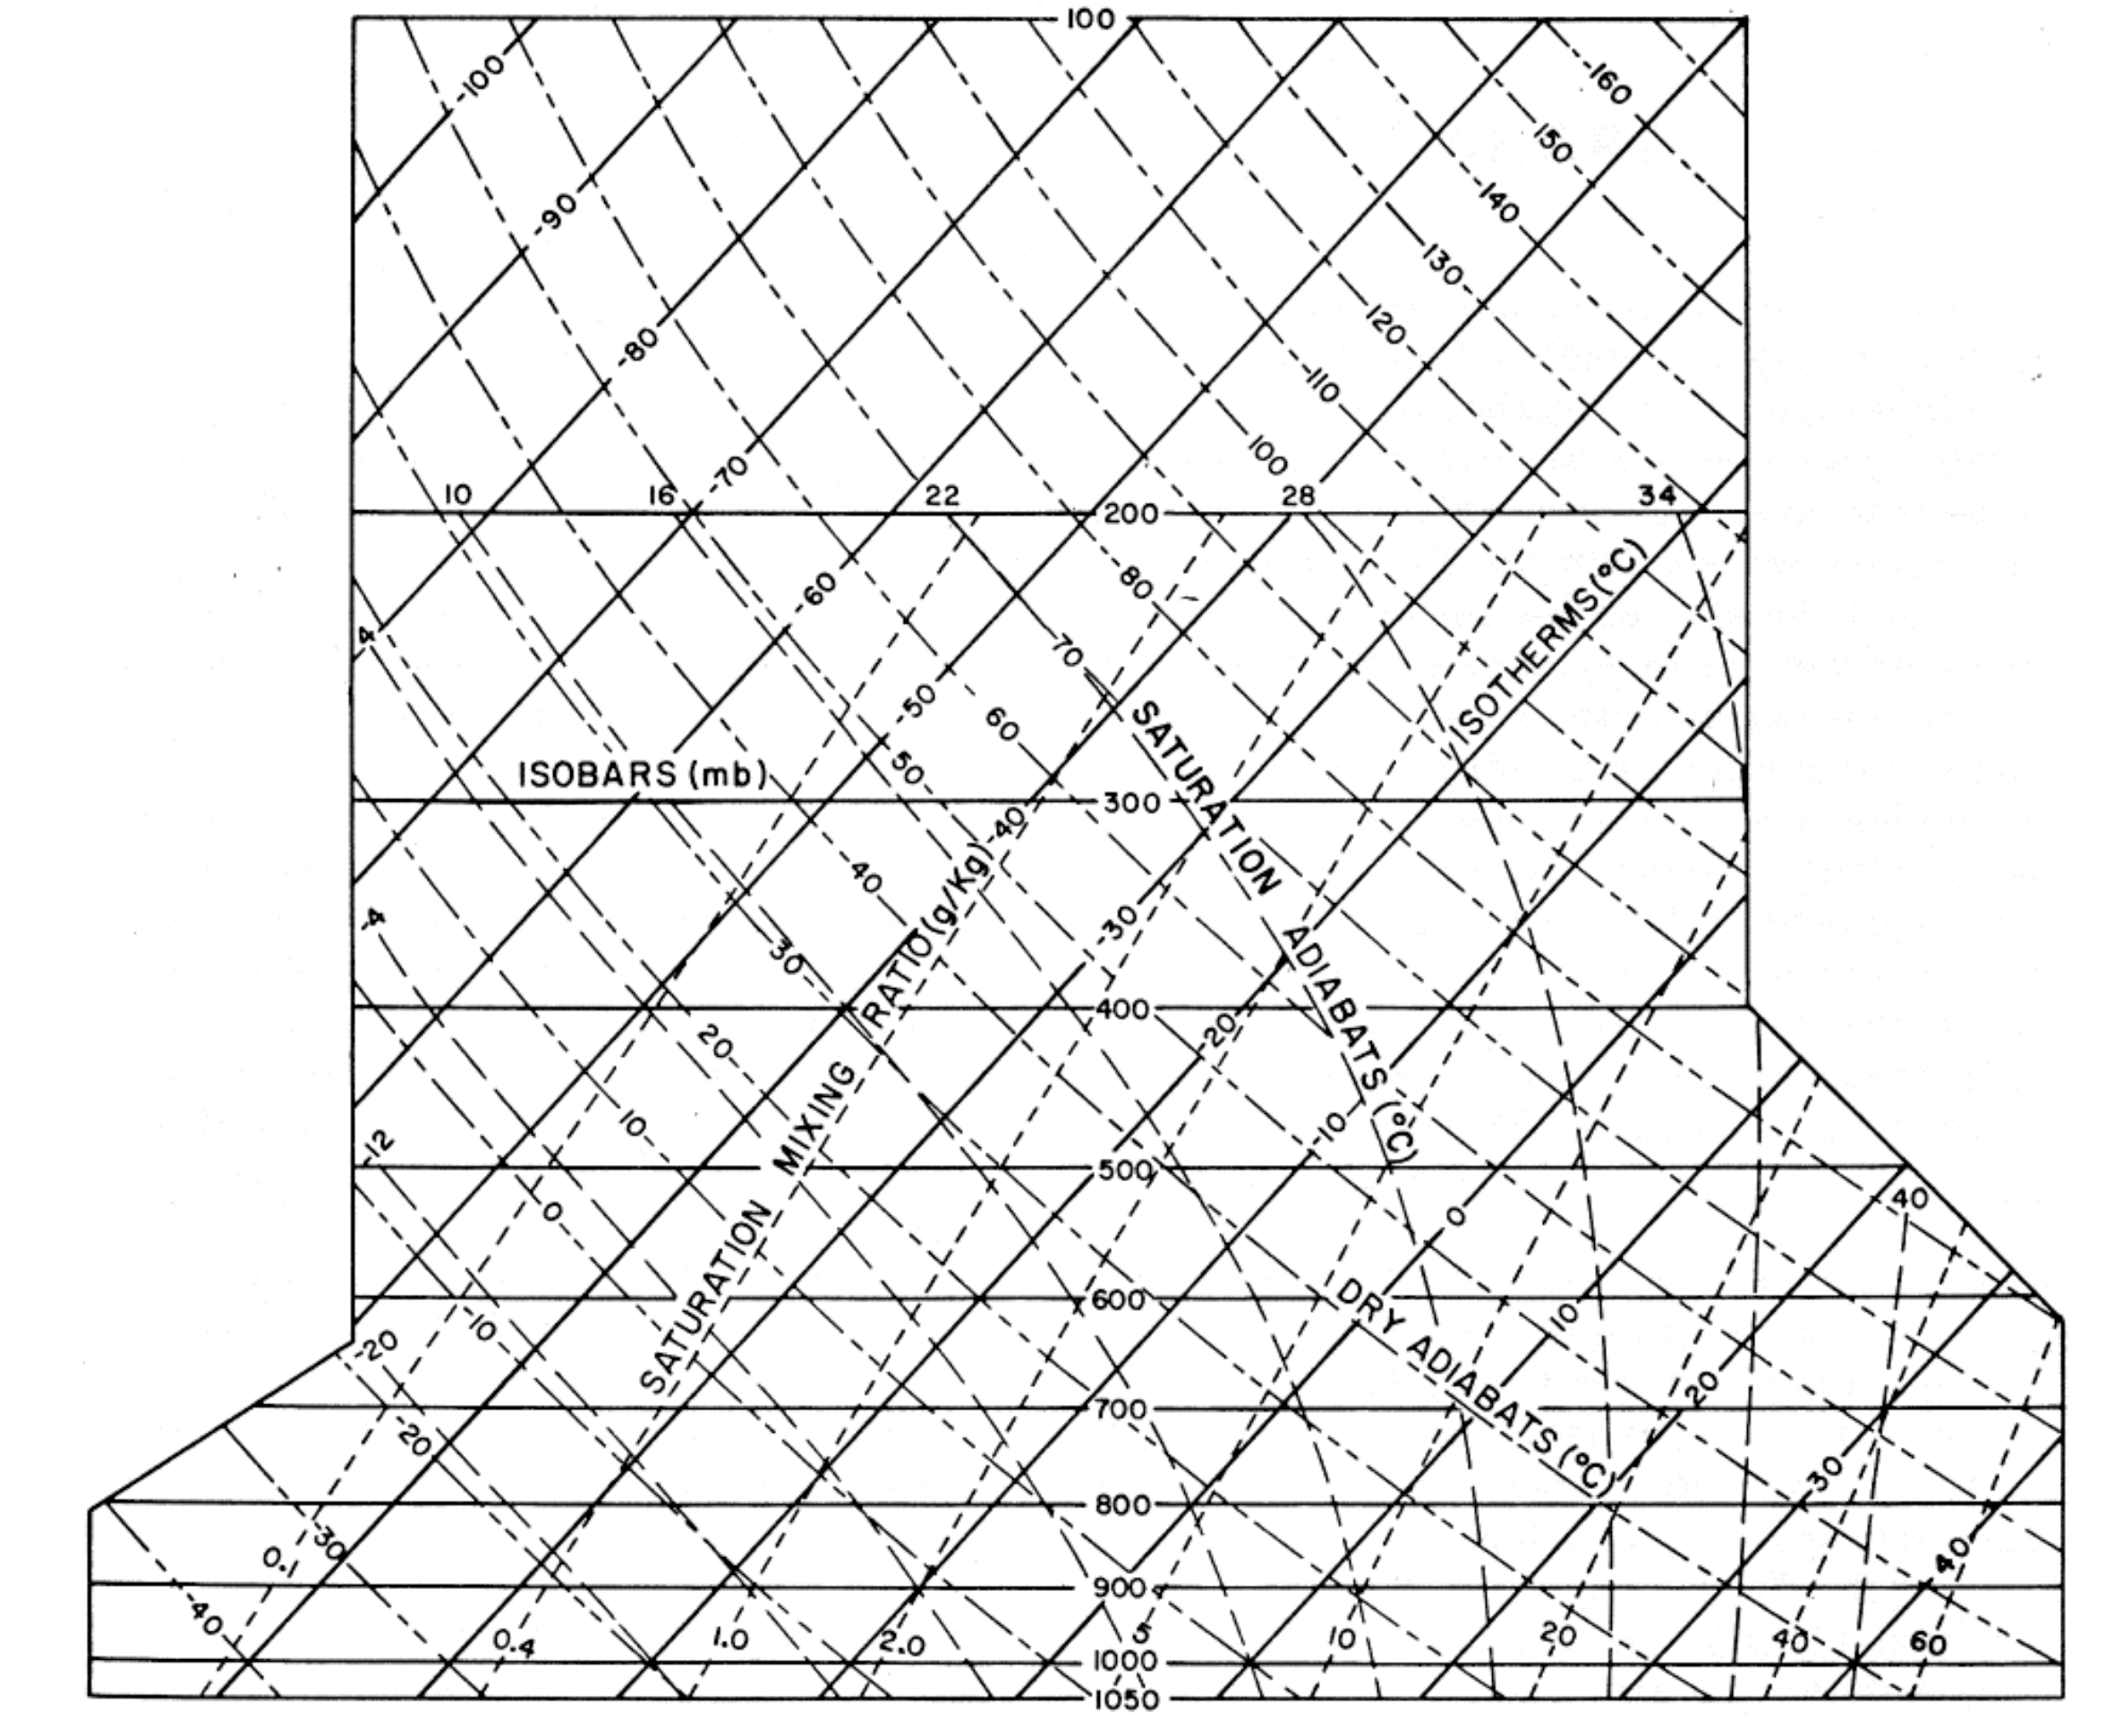
\includegraphics[width=0.8\textwidth]{fig3}
\end{figure}
\end{frame}

%------------------------------------------------

\begin{frame}{Atmospheric Thermodynamics: Adiabatic Processes}

\begin{itemize}
	\item Isobars
\end{itemize}
\begin{figure}
	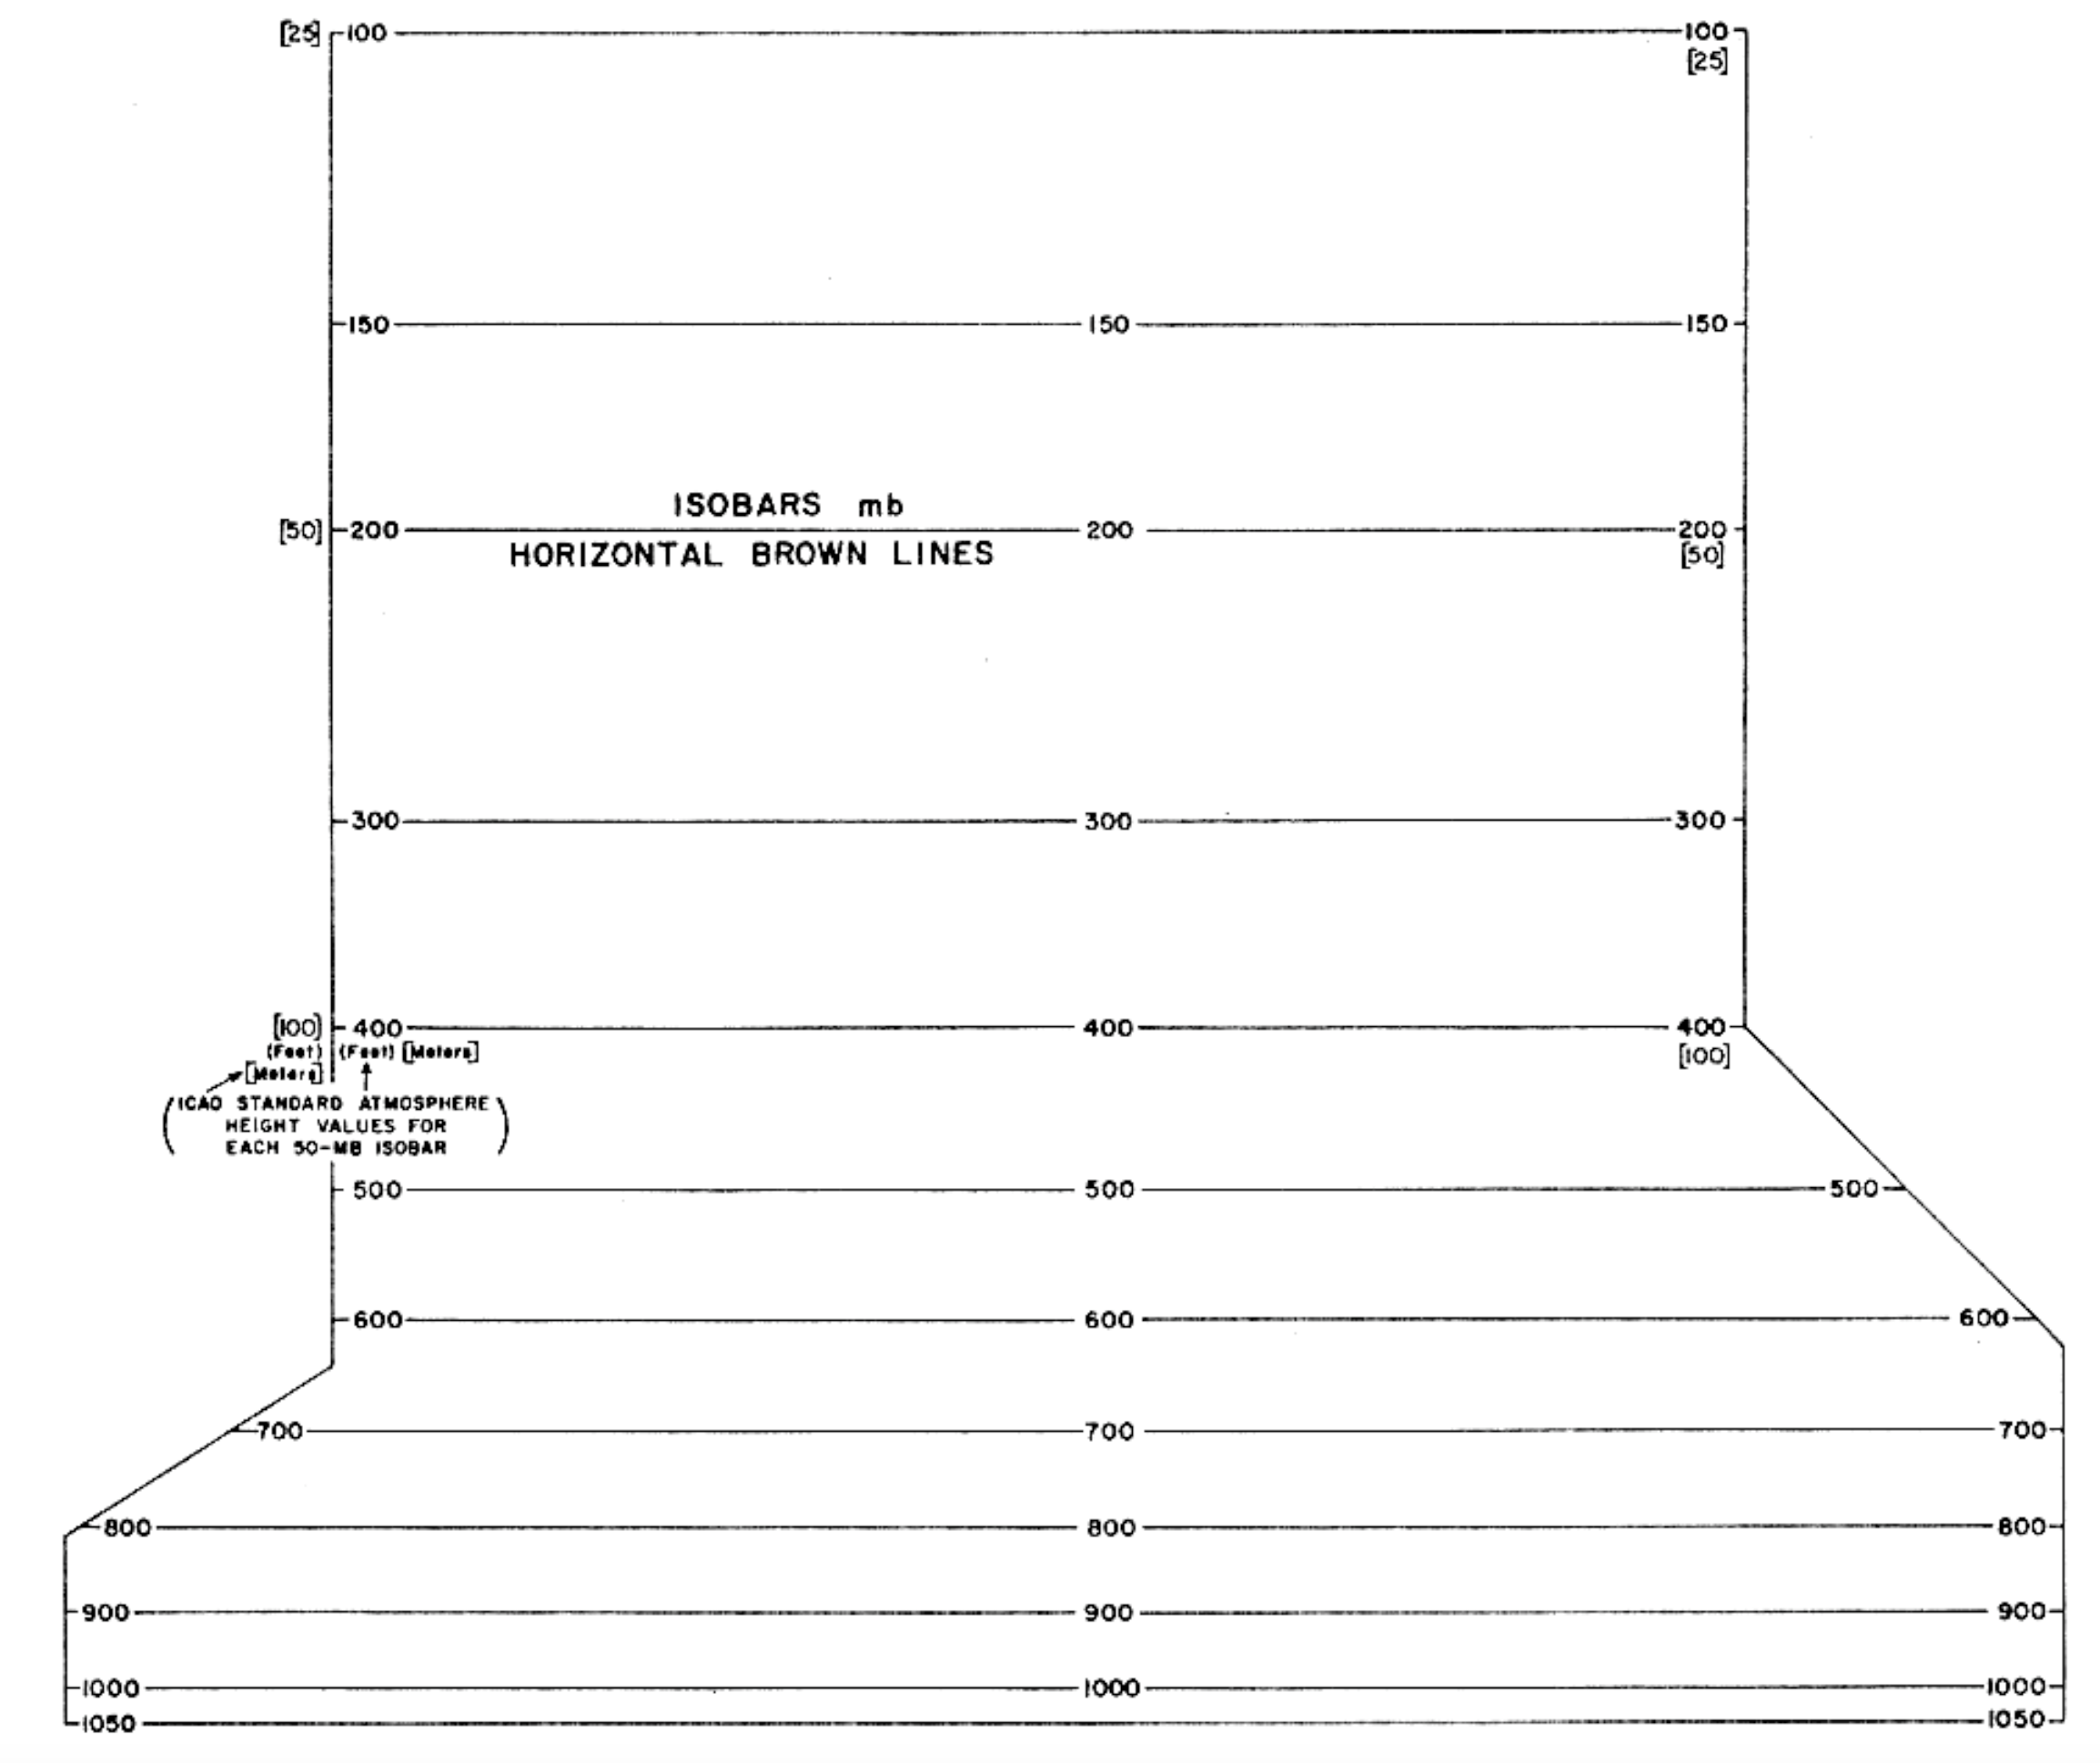
\includegraphics[width=0.8\textwidth]{fig4}
\end{figure}
\end{frame}

%------------------------------------------------

\begin{frame}{Atmospheric Thermodynamics: Adiabatic Processes}

\begin{itemize}
	\item Isotherms
\end{itemize}
\begin{figure}
	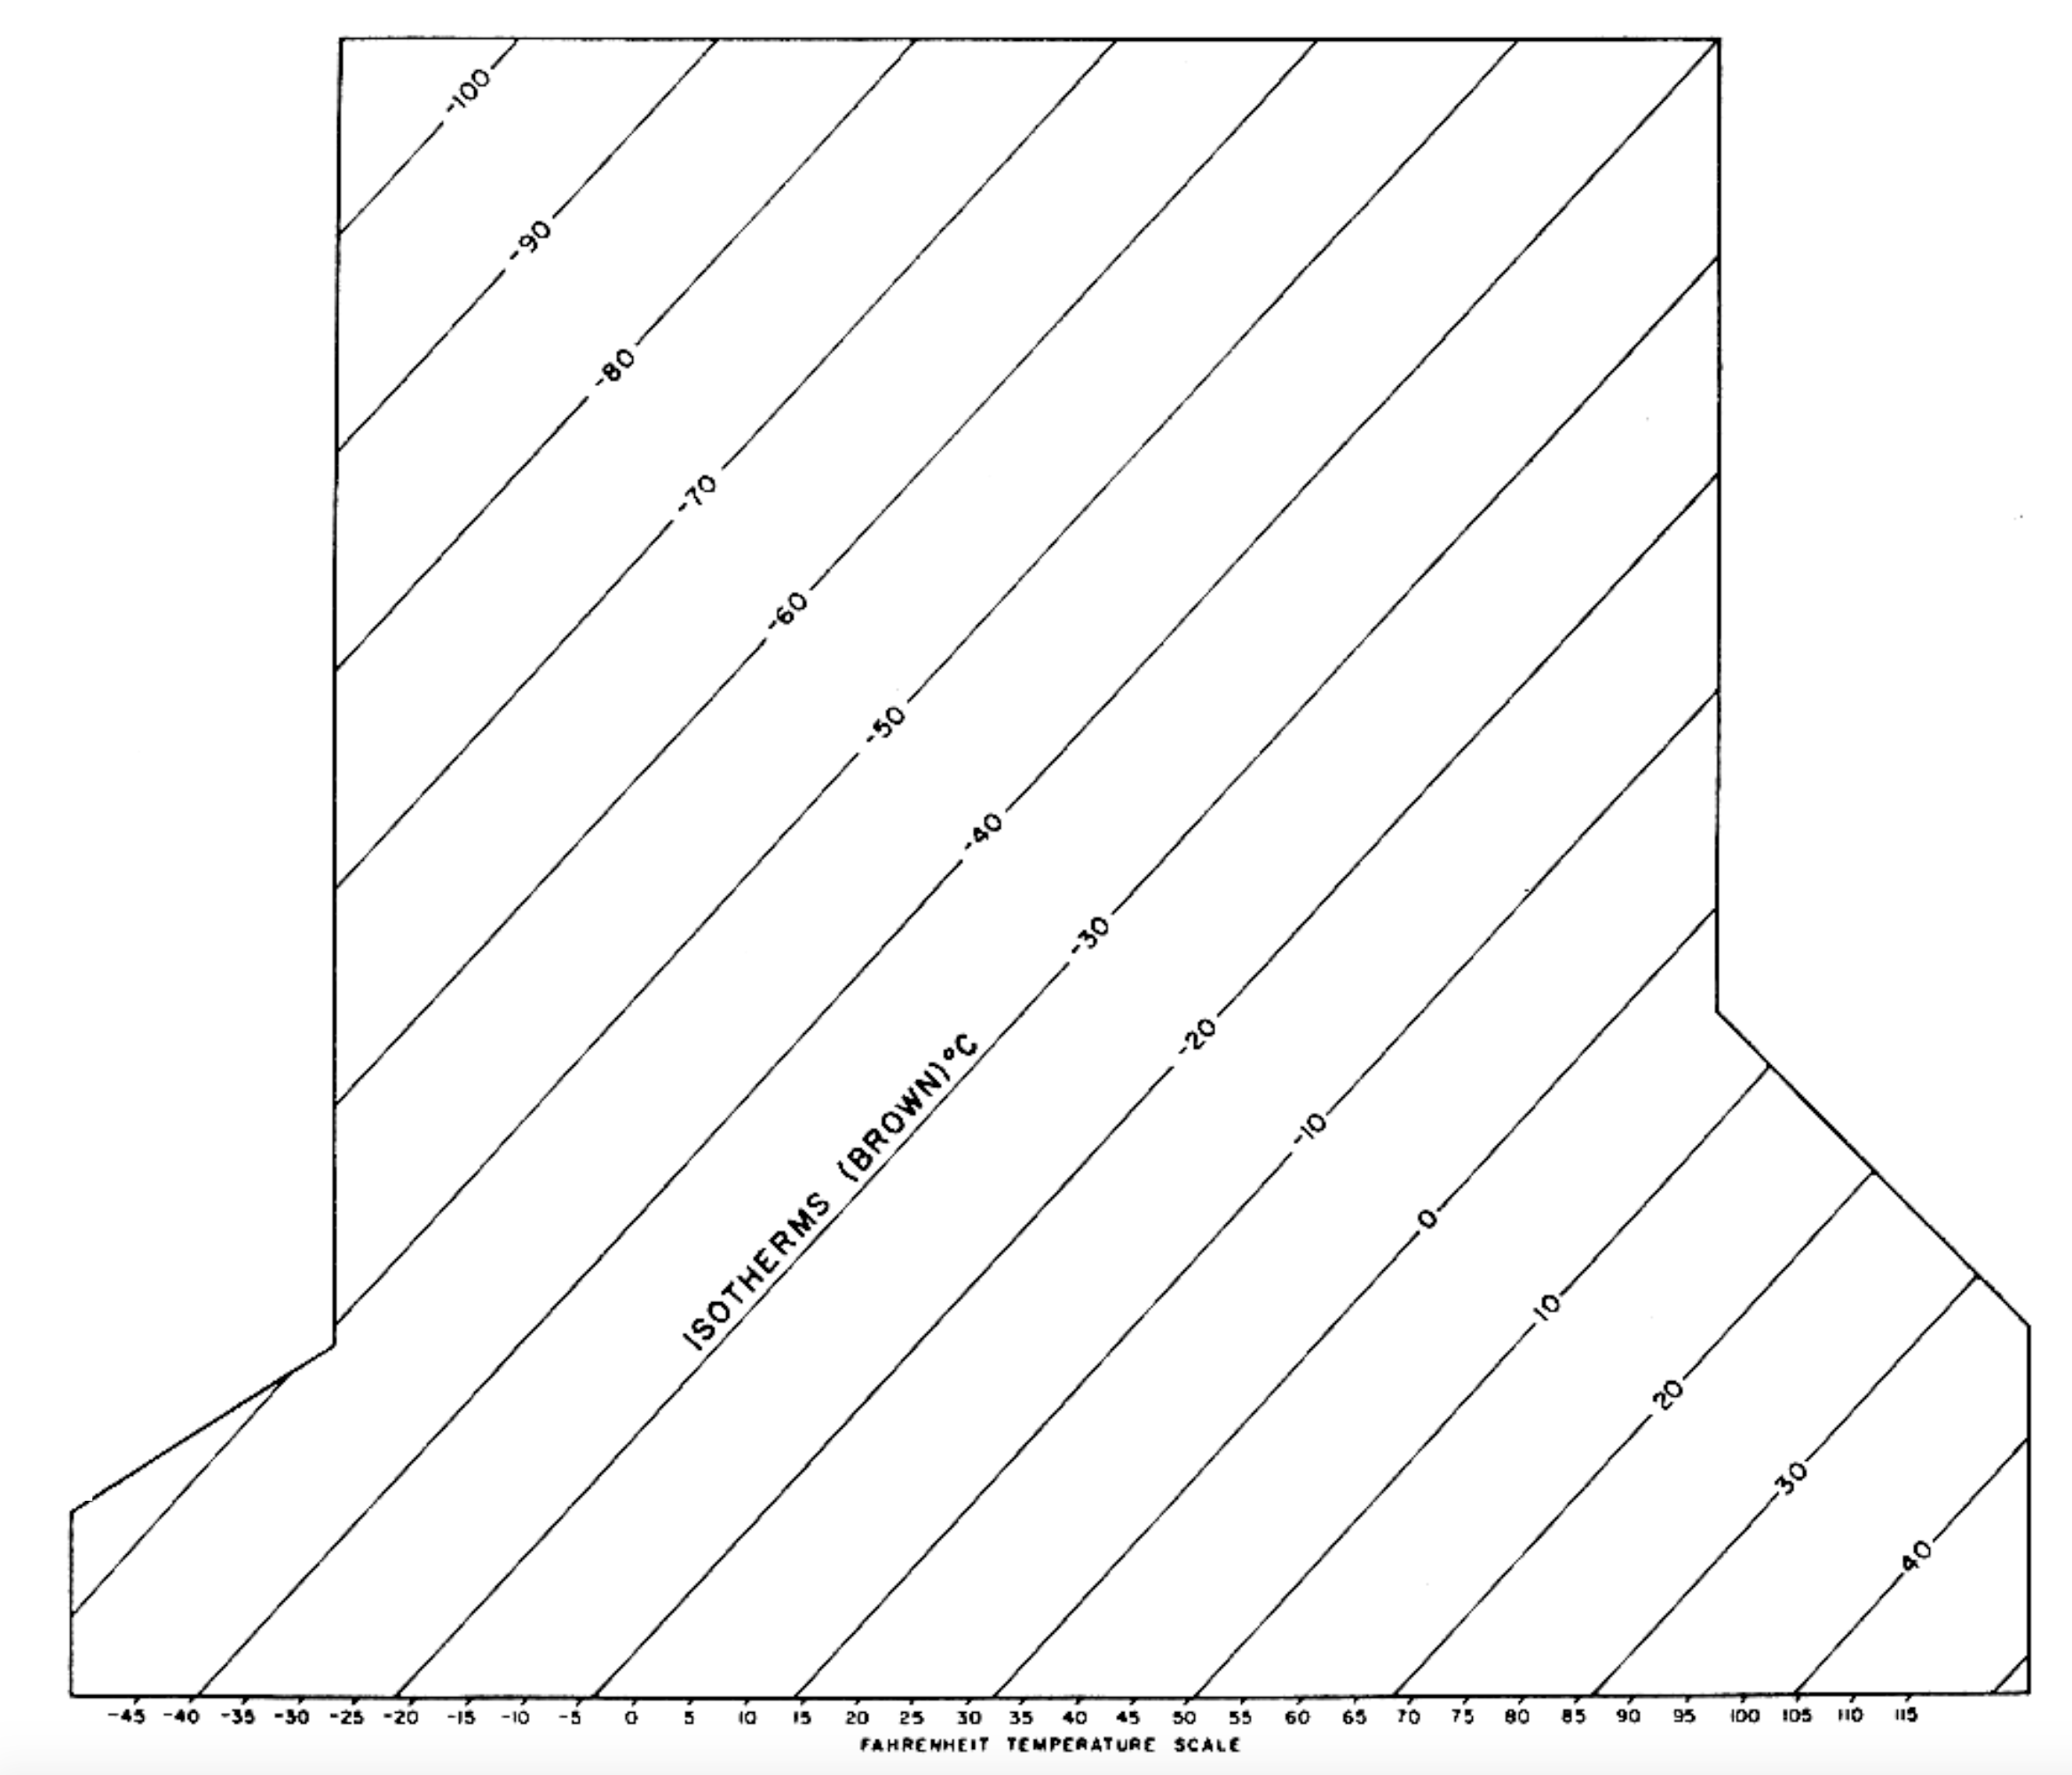
\includegraphics[width=0.8\textwidth]{fig5}
\end{figure}
\end{frame}

%------------------------------------------------

\begin{frame}{Atmospheric Thermodynamics: Adiabatic Processes}

\begin{itemize}
	\item Dry Adiabats
\end{itemize}
\begin{figure}
	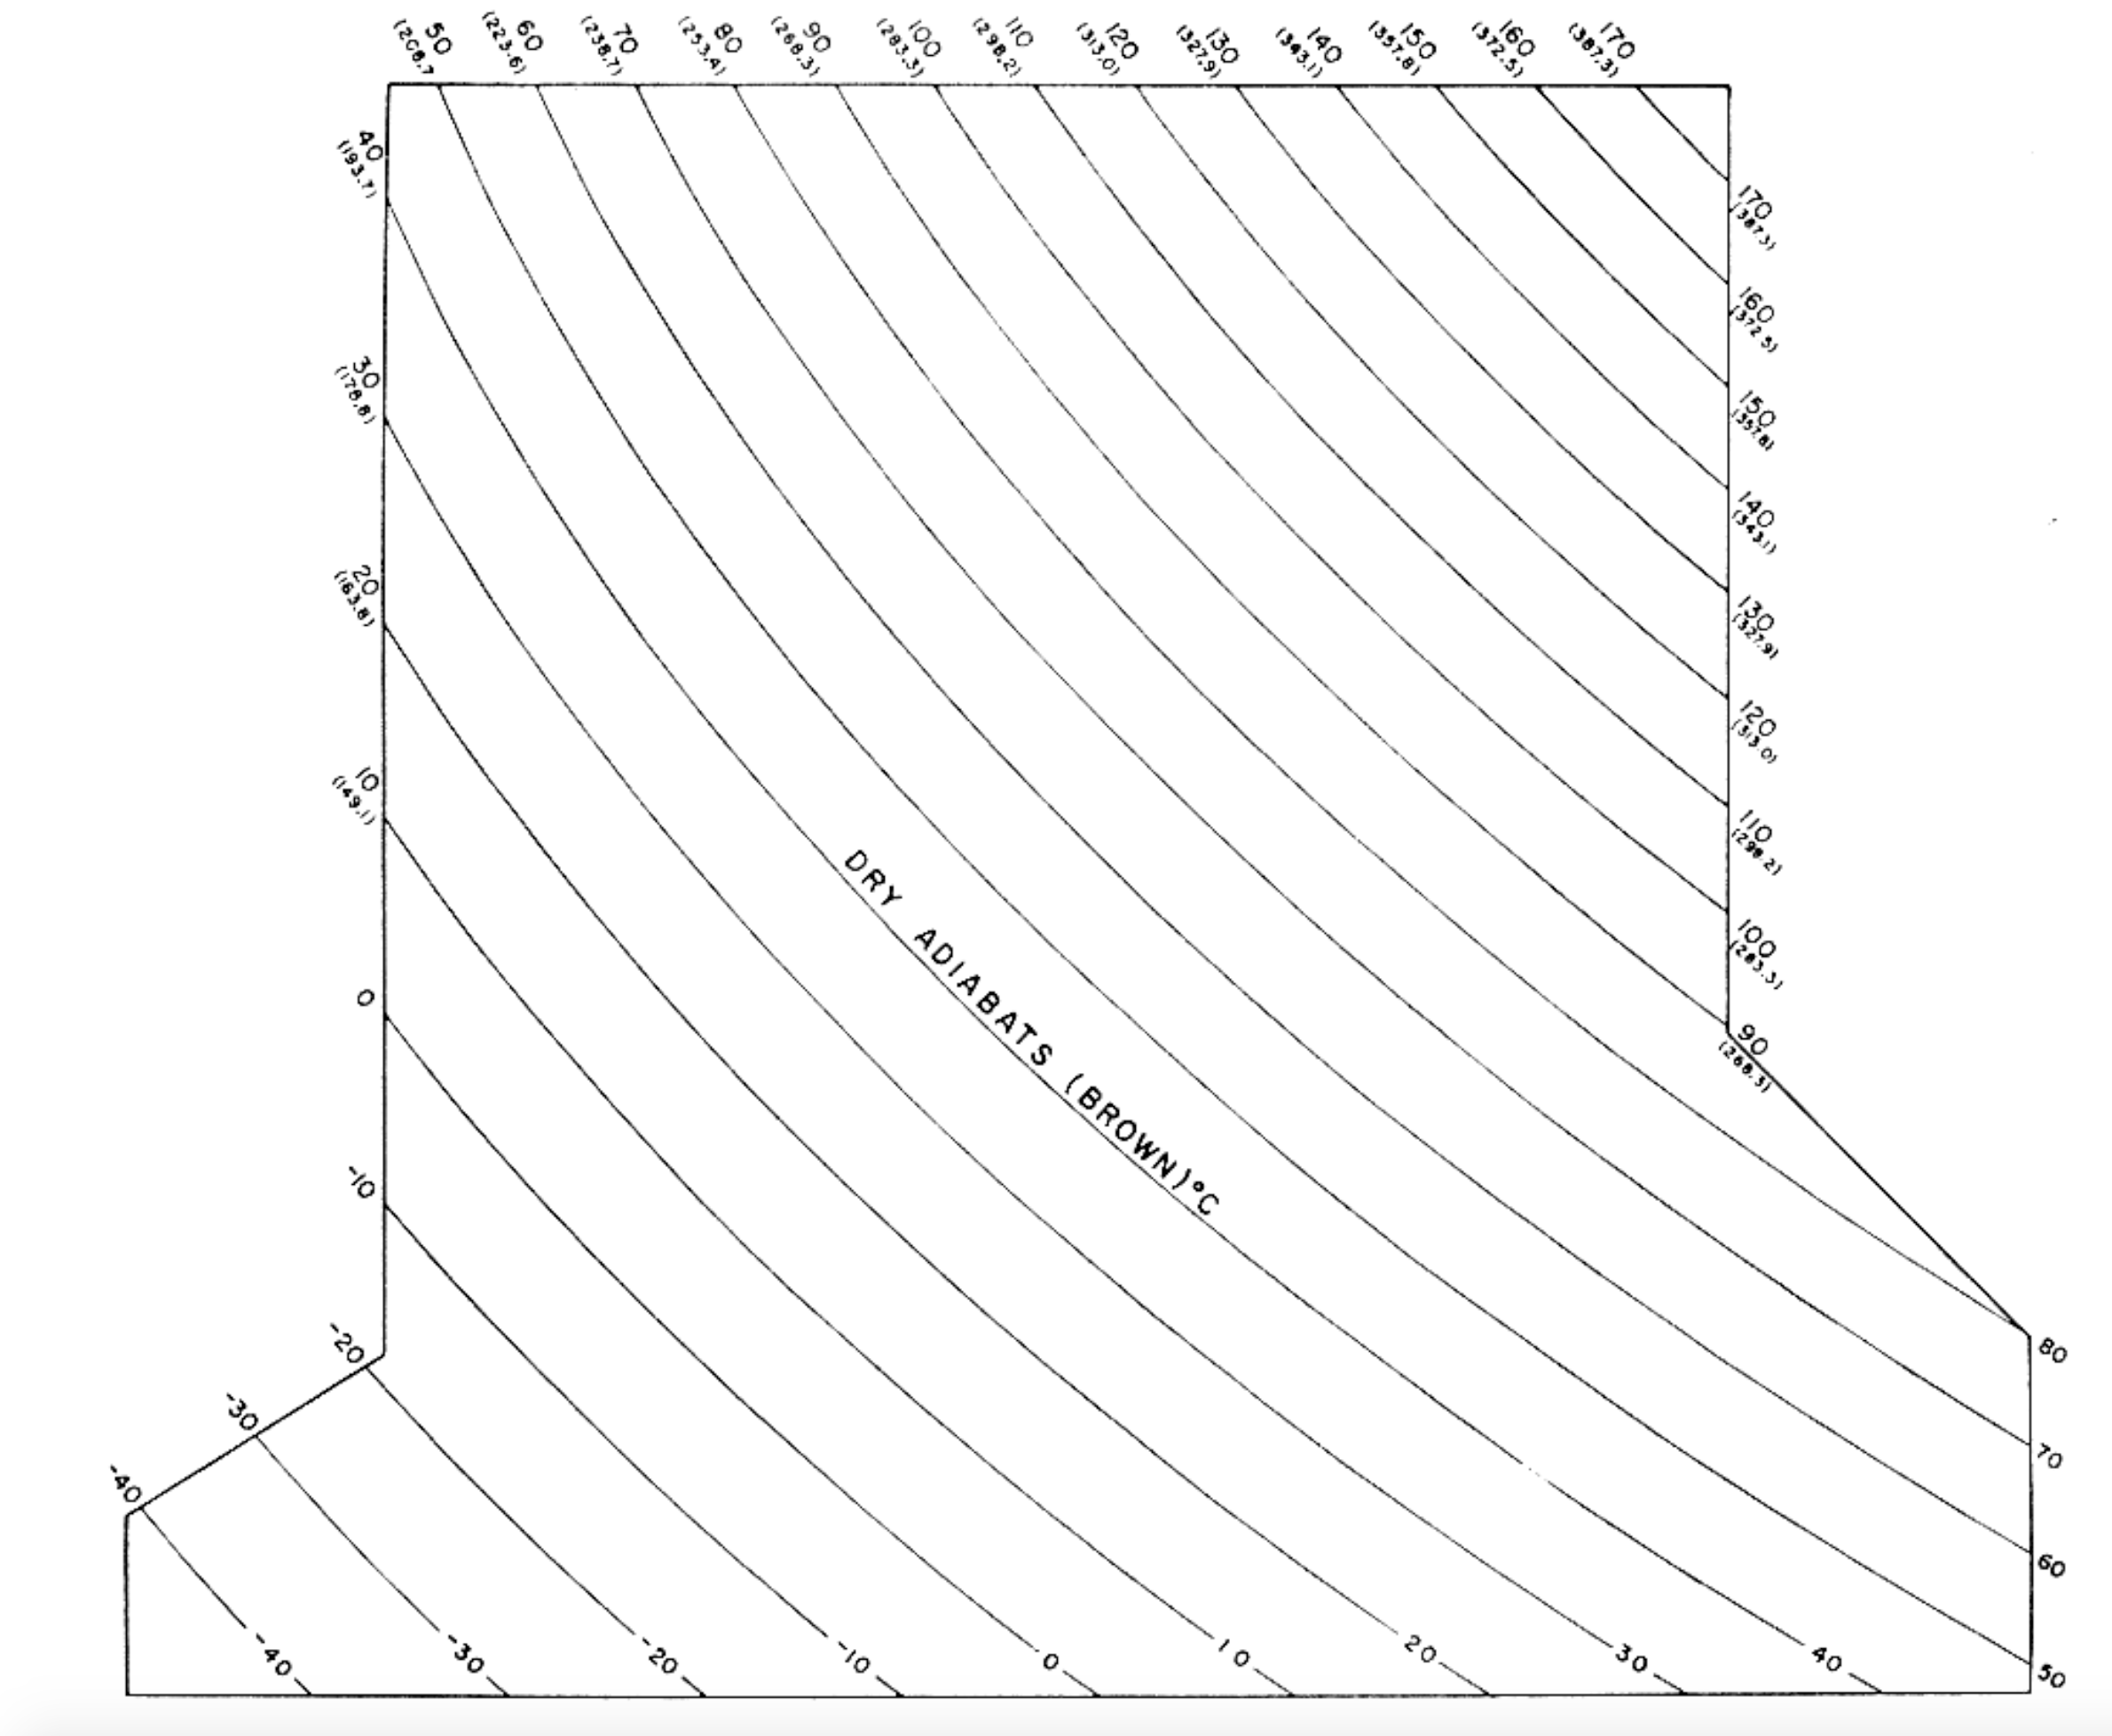
\includegraphics[width=0.8\textwidth]{fig6}
\end{figure}
\end{frame}

%------------------------------------------------

\begin{frame}{Atmospheric Thermodynamics: Adiabatic Processes}

\begin{itemize}
	\item Today's atmospheric sounding
\end{itemize}
\begin{figure}
	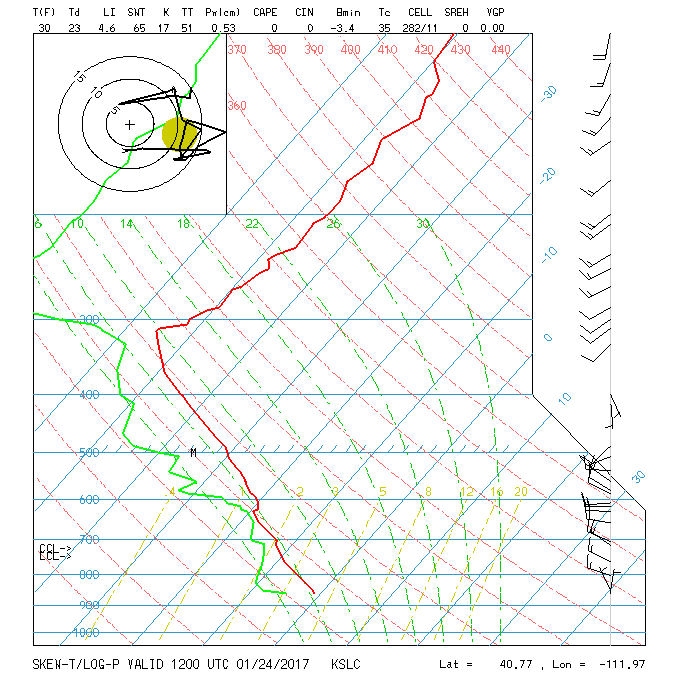
\includegraphics[width=0.7\textwidth]{fig7}
\end{figure}
\end{frame}

%------------------------------------------------



\end{document}

